\documentclass[aspectratio=169]{beamer}

\usepackage{mymacros}

\usepackage{graphicx}
  \graphicspath{{figures}}

\usetheme{firedrake}

\title{\texttt{pyop3} is coming}
\author{Connor Ward, David Ham, Jack Betteridge}
\date{16/09/2024}

\begin{document}

\frame{\titlepage}

\begin{frame}
  \begin{itemize}
    \item
      We have made a new package for \textbf{mesh stencil calculations}.
    \item
      It is called \pyop3.
    \item
      It will \textbf{soon replace} \pyop2 in Firedrake.
    \item
      This presentation will focus on the impact this will have on you, Firedrake users and developers.
    \item
      And hopefully inspire some of you to give it a try.
  \end{itemize}
\end{frame}

% Start by introducing PyOP2.
\begin{frame}{Introducing \pyop2}
  \vspace{-1em}
  \begin{center}
    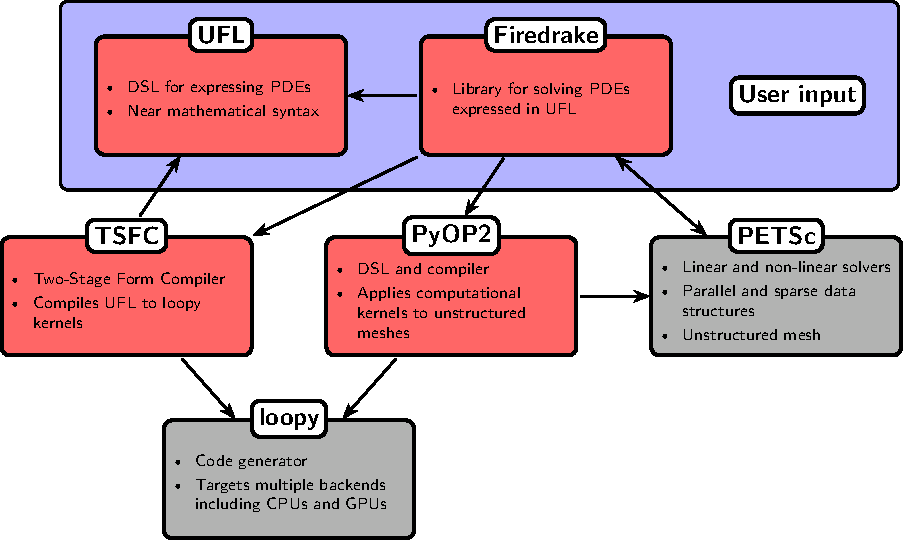
\includegraphics[width=.9\textwidth]{firedrake_structure_old.pdf}
  \end{center}
\end{frame}

\begin{frame}{Introducing \pyop2}
  \vspace{-2em}
  \begin{center}
    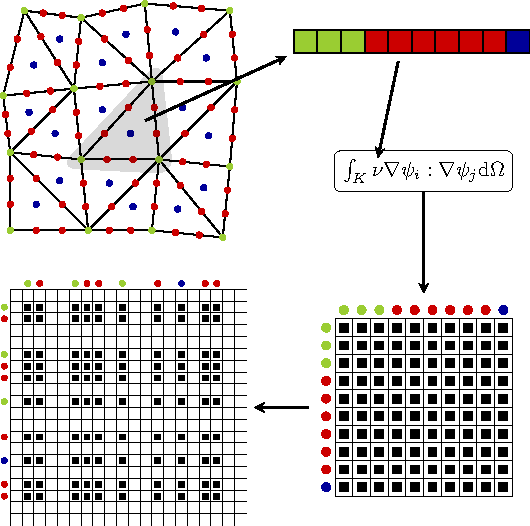
\includegraphics[scale=.9]{fem_assembly.pdf}
  \end{center}
\end{frame}

\begin{frame}{Why a mesh stencil abstraction?}
  \begin{itemize}
    \item 
      Writing one assembly loop is easy, writing many is hard.
    \item
      Changing algorithms and architectures mean that we need to be able to make high-level changes to various aspects of the computation.
      We don't want to write these all by hand.
    \item
      Also code generation is much faster than library functions.
  \end{itemize}
\end{frame}

\begin{frame}{Why do we need something new?}
  \pyop2 is a wonderful tool, but...

  \begin{itemize}
    \item
      It was designed specifically for FEM.
      More complex algorithms like additive-Schwartz methods (PCPatch) and hybridisation (SLATE) are possible but need hackery.
      This makes them inherently fragile.
    \pause
    \item
      It commits to one data layout, which is suboptimal in some circumstances.
  \end{itemize}
\end{frame}

\begin{frame}{Introducing \pyop3}
  \vspace{-2em}
  \begin{center}
    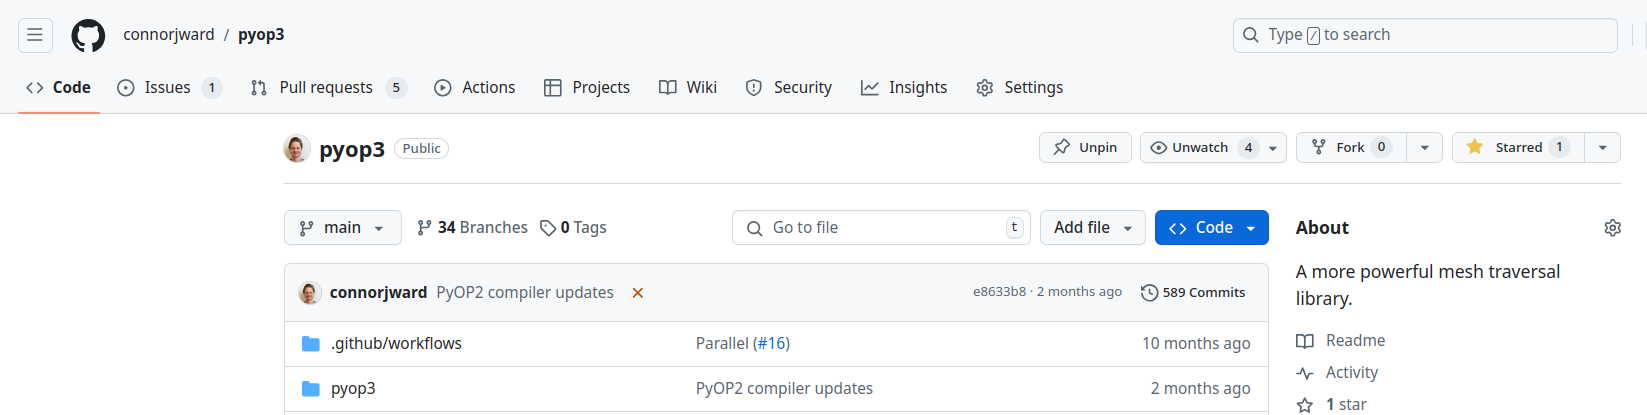
\includegraphics[width=\textwidth]{pyop3_github.png}
  \end{center}

  \begin{overprint}
    \onslide<1>\centering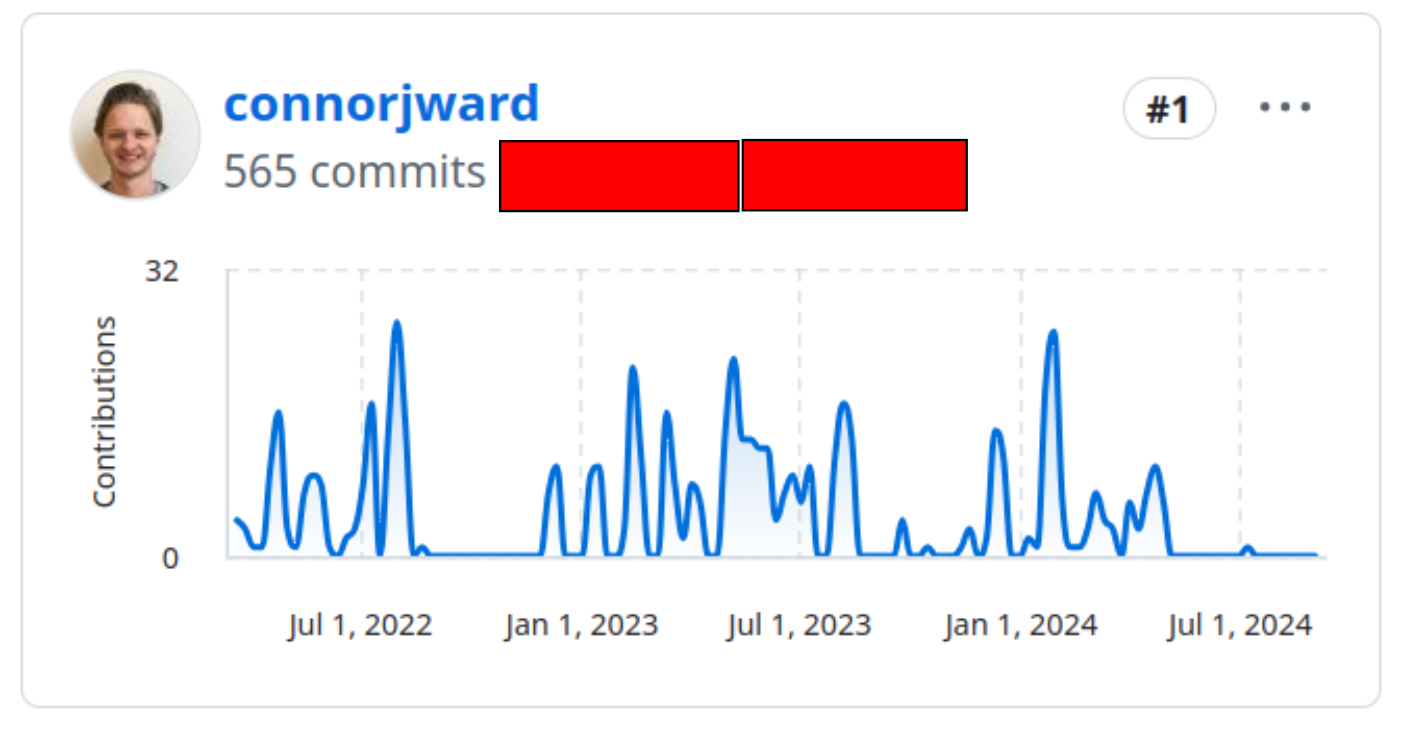
\includegraphics[width=.5\textwidth]{pyop3_github_stats_hidden.png}
    \onslide<2>\centering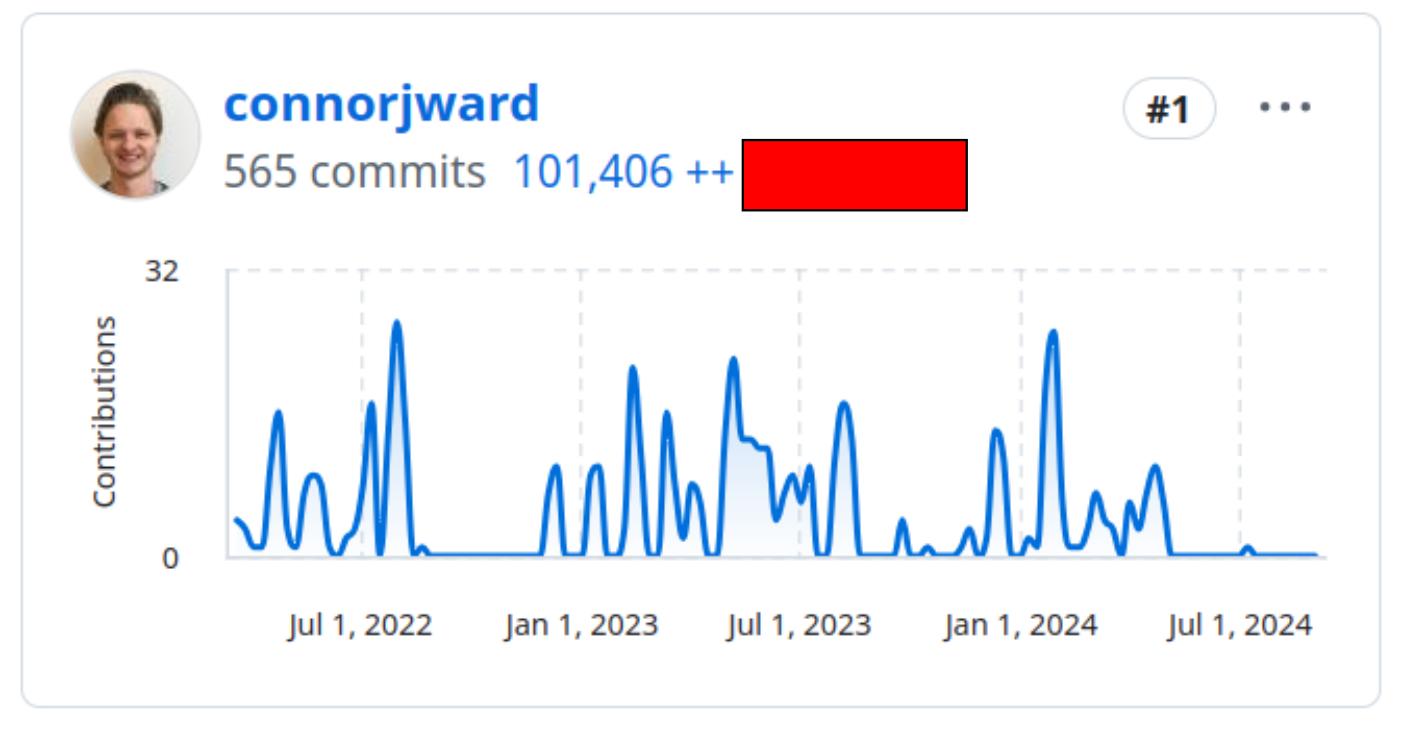
\includegraphics[width=.5\textwidth]{pyop3_github_stats_partial.png}
    \onslide<3>\centering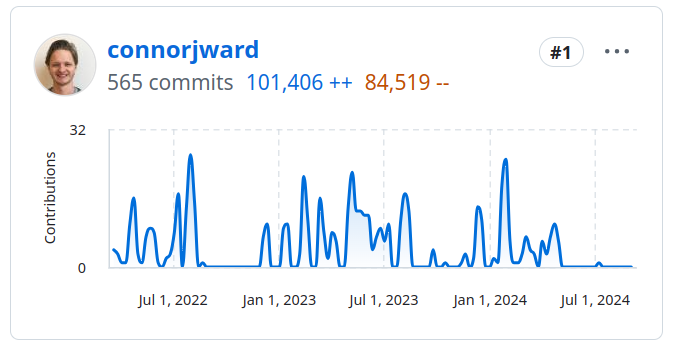
\includegraphics[width=.5\textwidth]{pyop3_github_stats_full.png}
  \end{overprint}
\end{frame}

\begin{frame}{An example: vertex-based slope limiter}
  % 2 columns, left is figure, right is pyop3 code
\end{frame}

\begin{frame}{An example: vertex-based slope limiter}
  % the generated C code
\end{frame}

\begin{frame}{Data layout transformations}
% ...
\end{frame}

\begin{frame}{Even more potential}
  \begin{itemize}
    \item
      preconditioners (SLATE, PCPatch)
% structured mesh
% other low-level compiler things (e.g. loop fusion)
% GPU!
  \end{itemize}
\end{frame}

\begin{frame}{Impact on Firedrake}
  \begin{itemize}
    \item
      Hopefully extremely minimal. The top-level API is unchanged.
    \item
      If you are frequently interacting directly with the arrays (i.e. \pycode{function.dat.data}) then you \emph{may} notice changes.
    \item
      Obviously any \pyop2 will need porting.
    \item
      Code performance may change (for better or worse).
      In principle shouldn't slow anything down.
  \end{itemize}
\end{frame}

\begin{frame}{Die, extruded mesh! Die! Die! Die!}
  % extreme case of premature optimisation
  % discuss performance and feature implications
\end{frame}

\begin{frame}{What next?}
  \pause
  \vspace{-3em}
  
\includegraphics[width=\textwidth]{shark.png}
\end{frame}

\begin{frame}{But then?}
  \begin{itemize}
    \item
      \pyop3 should be merged within the next 6 months.
    \item
      It will be in a usable state well before then.
    \item
      Hopefully then we will have funding for me to get it working on GPUs.
  \end{itemize}
\end{frame}

\end{document}
